\documentclass[border=14pt]{standalone}
\usepackage[T1]{fontenc}
\usepackage[scaled]{helvet}
\renewcommand\familydefault\sfdefault
\usepackage{tikz}
\usetikzlibrary{arrows.meta,calc,positioning}
\definecolor{personF}{HTML}{F8E0A8}\definecolor{personD}{HTML}{B8860B}
\definecolor{slackF}{HTML}{DCE8F6}\definecolor{slackD}{HTML}{5B7FA8}
\definecolor{sessF}{HTML}{CDE8E1}\definecolor{sessD}{HTML}{2E8B74}
\definecolor{subF}{HTML}{E6DDF3}\definecolor{subD}{HTML}{7E5DB8}
\definecolor{workF}{HTML}{E1EECD}\definecolor{workD}{HTML}{6A9A3A}
\definecolor{servF}{HTML}{E6E8EB}\definecolor{servD}{HTML}{8A9099}
\definecolor{codeF}{HTML}{F6DAD6}\definecolor{codeD}{HTML}{C0605A}
\definecolor{arrC}{HTML}{6B7280}\definecolor{labC}{HTML}{555B66}
\tikzset{
  box/.style={rounded corners=3pt, draw, line width=0.8pt, align=center, text width=3.4cm,
              inner sep=5pt, minimum height=1.2cm, font=\normalsize},
  person/.style={box, fill=personF, draw=personD},
  slack/.style={box, fill=slackF, draw=slackD},
  sess/.style={box, fill=sessF, draw=sessD},
  sub/.style={box, fill=subF, draw=subD},
  work/.style={box, fill=workF, draw=workD},
  serv/.style={box, fill=servF, draw=servD},
  code/.style={box, fill=codeF, draw=codeD},
  arr/.style={-{Stealth[length=2.4mm,width=1.8mm]}, draw=arrC, line width=0.8pt},
  lab/.style={font=\small\itshape, text=labC, fill=white, inner sep=1.5pt},
}
\hyphenpenalty=10000 \exhyphenpenalty=10000
\newcommand\nd[2]{\textbf{#1}\\[1pt]{\small #2}}
\newcommand\titled[2]{\node[anchor=south west, inner sep=0pt] at ($(current bounding box.north west)+(0cm,0.45cm)$)
  {{\bfseries\LARGE #1}\hspace{1.2em}{\color{labC}\large #2}};}
\begin{document}
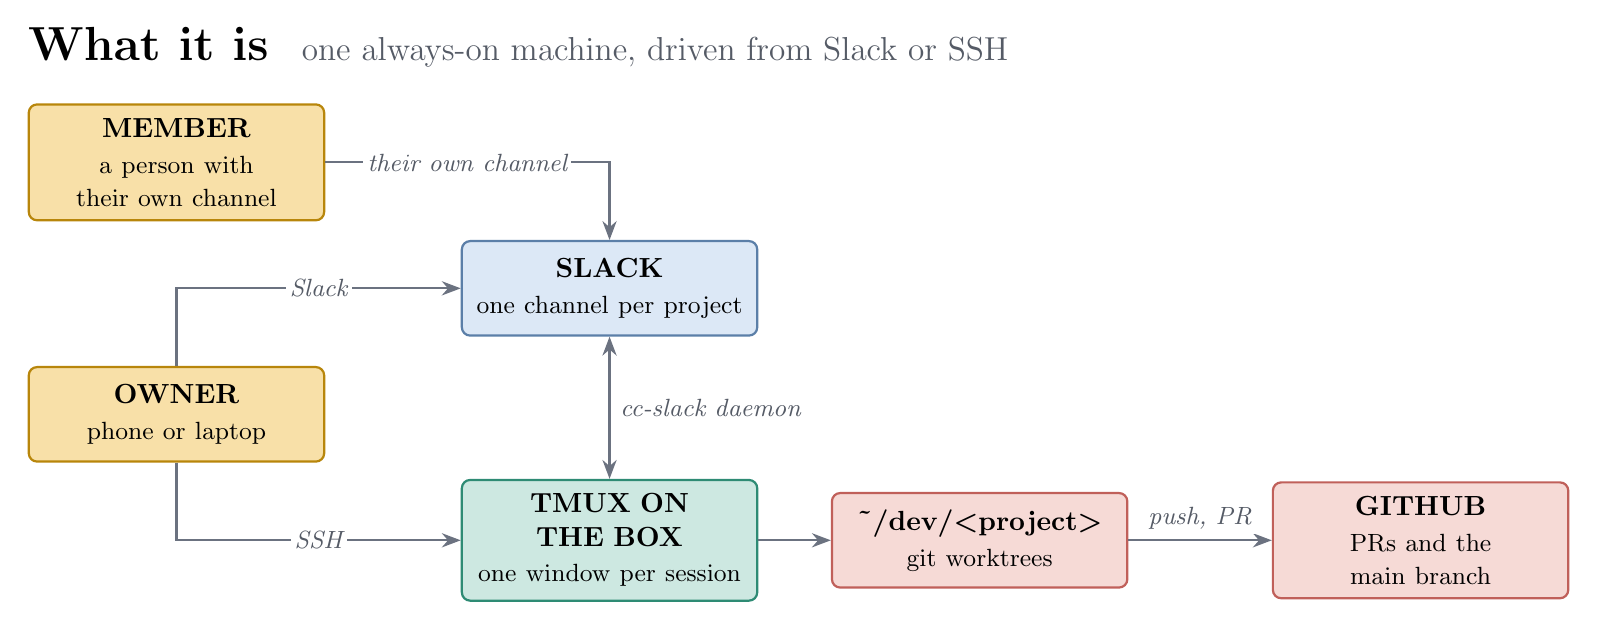
\begin{tikzpicture}
\node[person] (member) at (0,3.2) {\nd{MEMBER}{a person with their own channel}};
\node[person] (owner) at (0,0) {\nd{OWNER}{phone or laptop}};
\node[slack] (slack) at (5.5,1.6) {\nd{SLACK}{one channel per project}};
\node[sess] (tmux) at (5.5,-1.6) {\nd{TMUX ON THE BOX}{one window per session}};
\node[code] (repos) at (10.2,-1.6) {\nd{\textasciitilde/dev/\textless project\textgreater}{git worktrees}};
\node[code] (gh) at (15.8,-1.6) {\nd{GITHUB}{PRs and the main branch}};
\draw[arr] (owner.north) |- node[lab, pos=0.75] {Slack} (slack.west);
\draw[arr] (owner.south) |- node[lab, pos=0.75] {SSH} (tmux.west);
\draw[arr] (member.east) -| node[lab, pos=0.25] {their own channel} (slack.north);
\draw[arr, {Stealth[length=2.4mm,width=1.8mm]}-{Stealth[length=2.4mm,width=1.8mm]}] (slack.south) -- node[lab, right=2pt] {cc-slack daemon} (tmux.north);
\draw[arr] (tmux) -- (repos);
\draw[arr] (repos) -- node[lab, above=2pt] {push, PR} (gh);
\titled{What it is}{one always-on machine, driven from Slack or SSH}
\end{tikzpicture}
\end{document}
